\section{Основни принципи, технологии и развойни среди за реализация на мобилни приложения}
\subsection{Мобилно приложение}
Мобилното приложение е компютърна програма, създадена, за да работи на мобилни устройства като смартфони и таблети. Най-често срещаните мобилни операционни системи са Android на Google и iOS на Apple Inc. Обикновено приложенията са достъпни на онлайн платформи за диситрибуция като App Store, Google Play Store, Galaxy Store и др. Обикновено платформата е построена и се оправлява от компанията собственик на операционната система на устройството.

\subsection{Езици за програмиране на Android приложения}
Приложенията за Android могат да се пишат на езиците Kotlin, Java и C++, с помощта на комплекта за разработка на софтуер за Android - Android SDK, като същевременно е възможно и използване на други езици. Всички езици, които не са използват виртуалната машина Java (напр.: Go, JavaScript, C и т.н.) се нуждаят от помощта на интерпретатор.

\subsection{Езици за програмиране на iOS приложения}
При разработката на мобилно iOS приложение освен популярните езици базирани на C (C++/C\#) се използва и Swift. Swift e програмен език със свободен код, създаден през 2014 от Apple Inc. специално за разработка на iOS приложения. Базиран е на езикът C и е разработен така че да има огромен спектър на функционалност, тъй като светът на мобилните приложения е много широк. Swift е компилируем език, който се характеризира с това, че превръщат програмния код в машинен.

\subsection{Езици за междуплатформени приложения}
Когато се отнася до мобилно програмиране, има налични софтуерни рамки, които предоставят възможността за разработка едновременно и за двете гореспоменати мобилни платформи. Примери за това са Flutter, React Native, Xamarin и други. При подобен софтуер за разработка от една кодова база се компилира приложение за много платформи.

Flutter е комплект за разработка на софтуер за потребителски интерфейс с отворен код, създаден от Google. Използва се за разработване на крос-платформени приложения за Android, iOS, Linux, Mac, Windows, Google Fuchsia, както и на уеб страници от единна кодова база. Flutter използва обектно-ориентирания език Dart при разработка, който също е създаден от Google.

React Native е софтуерна рамка за потребителски интерфейс с отворен код, създадена от Facebook, Inc. Използва се за разработване на приложения за Android, Android TV, iOS, macOS tvOS, Web, Windows и UWP, като дава възможност на разработчиците да използват рамката React заедно с локалните за мобилното устройство функционалности. Често случаи е предпочитана от хора и организации, които се занимават с програмирането на уеб приложения на React, поради голямата сходност между технологиите.

\subsection{Развойни среди за разработка на мобилни приложения}
Основната среда за разработка на Android приложения е Android Studio. Android Studio е разширение на IntelliJ IDEA редактора на JetBrains и се използва едининствено за разработката на мобилни приложения. Редактора предоставя множество инструменти, като Android SDK, Android Virtual Device (ADV) и д.р., които да улеснят работата на разработчиците. (Фиг. \ref{fig:screenshot-android-studio})

\begin{figure}[H]
    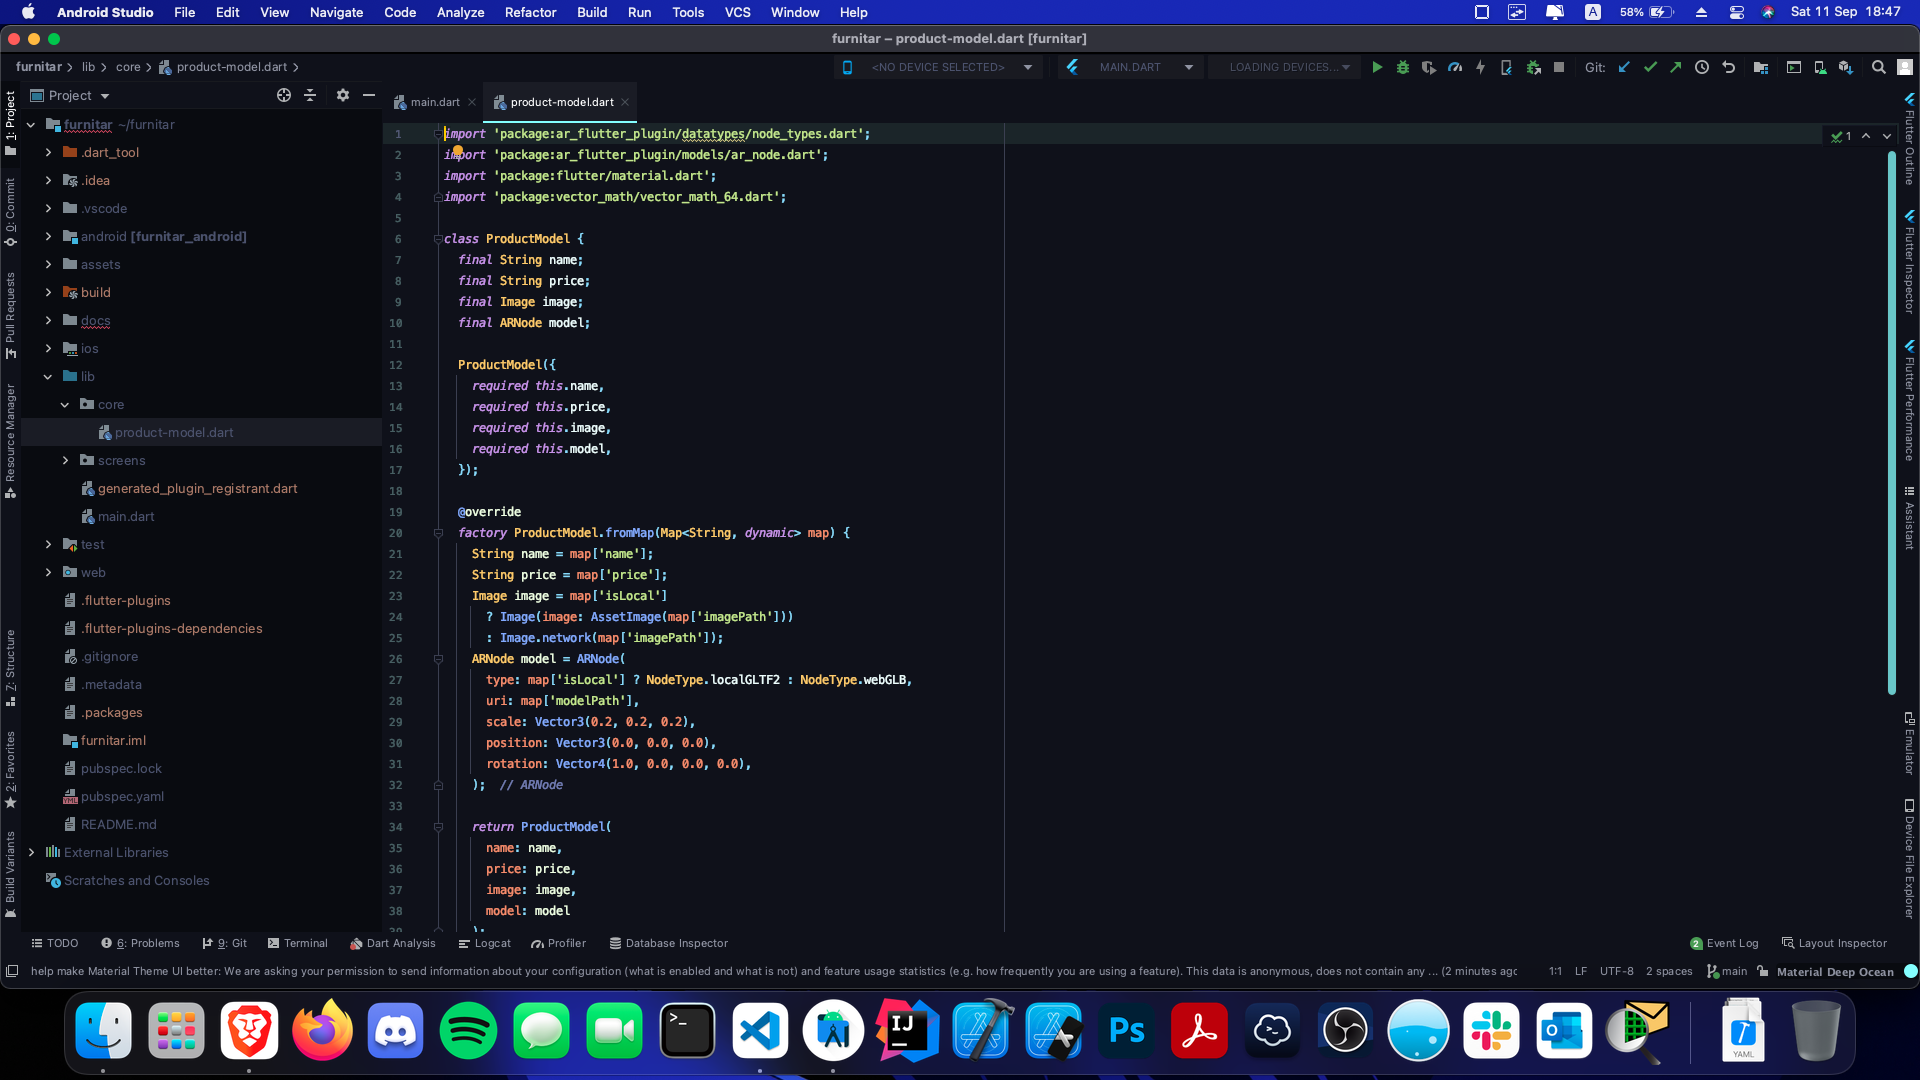
\includegraphics[width=1\textwidth]{screenshot-android-studio.png}
    \centering
    \caption{Снимка от Android Studio}
    \label{fig:screenshot-android-studio}
\end{figure}

Основната среда за разработка на iOS приложения на е Xcode. Xcode е платформа, създадена от Apple Inc., ексклузивно за разработването на приложения и програми за устройства, използващи операционните системи на компанията. Тази платформа се използва масово, защото функционалността на платформата е максимално съвместима с операционните системи на компанията, изграждайки много добра връзка между устройството и кода. Xcode също така предоставя симулации на голяма част от мобилните устройства на компанията, което значително улеснява разработката на приложения за тях. (Фиг. \ref{fig:screenshot-xcode})

\begin{figure}[H]
    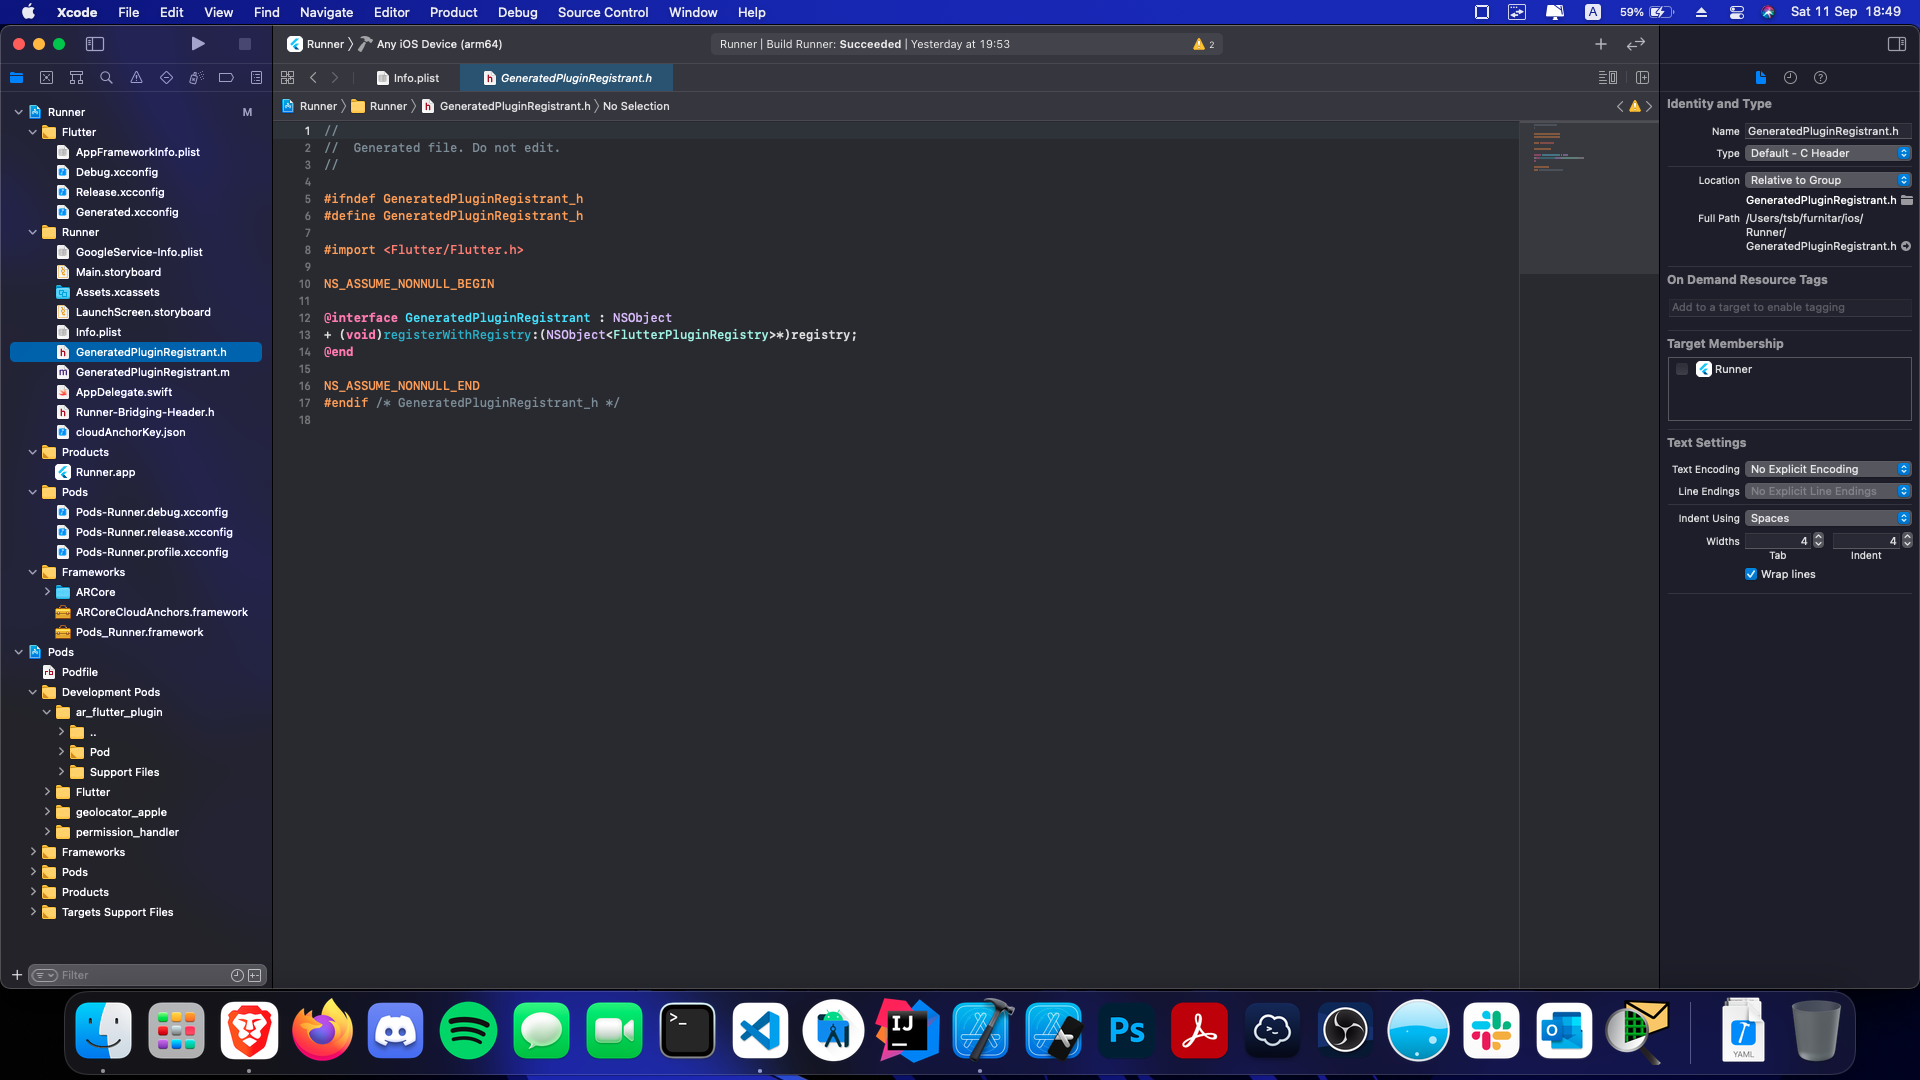
\includegraphics[width=1\textwidth]{screenshot-xcode.png}
    \centering
    \caption{Снимка от XCode}
    \label{fig:screenshot-xcode}
\end{figure}

Visual Studio Code е интегрирана среда за разработка, направена от Microsoft за Windows, Linux и macOS. Характеристиките включват поддръжка за отстраняване на грешки, подчертаване на синтаксиса, интелигентно завършване на код, фрагменти, рефакторинг на код и вграден Git. Потребителите могат да променят темата, клавишните комбинации, предпочитанията и да инсталират разширения, които добавят допълнителна функционалност. (Фиг. \ref{fig:screenshot-vscode})

\begin{figure}[H]
    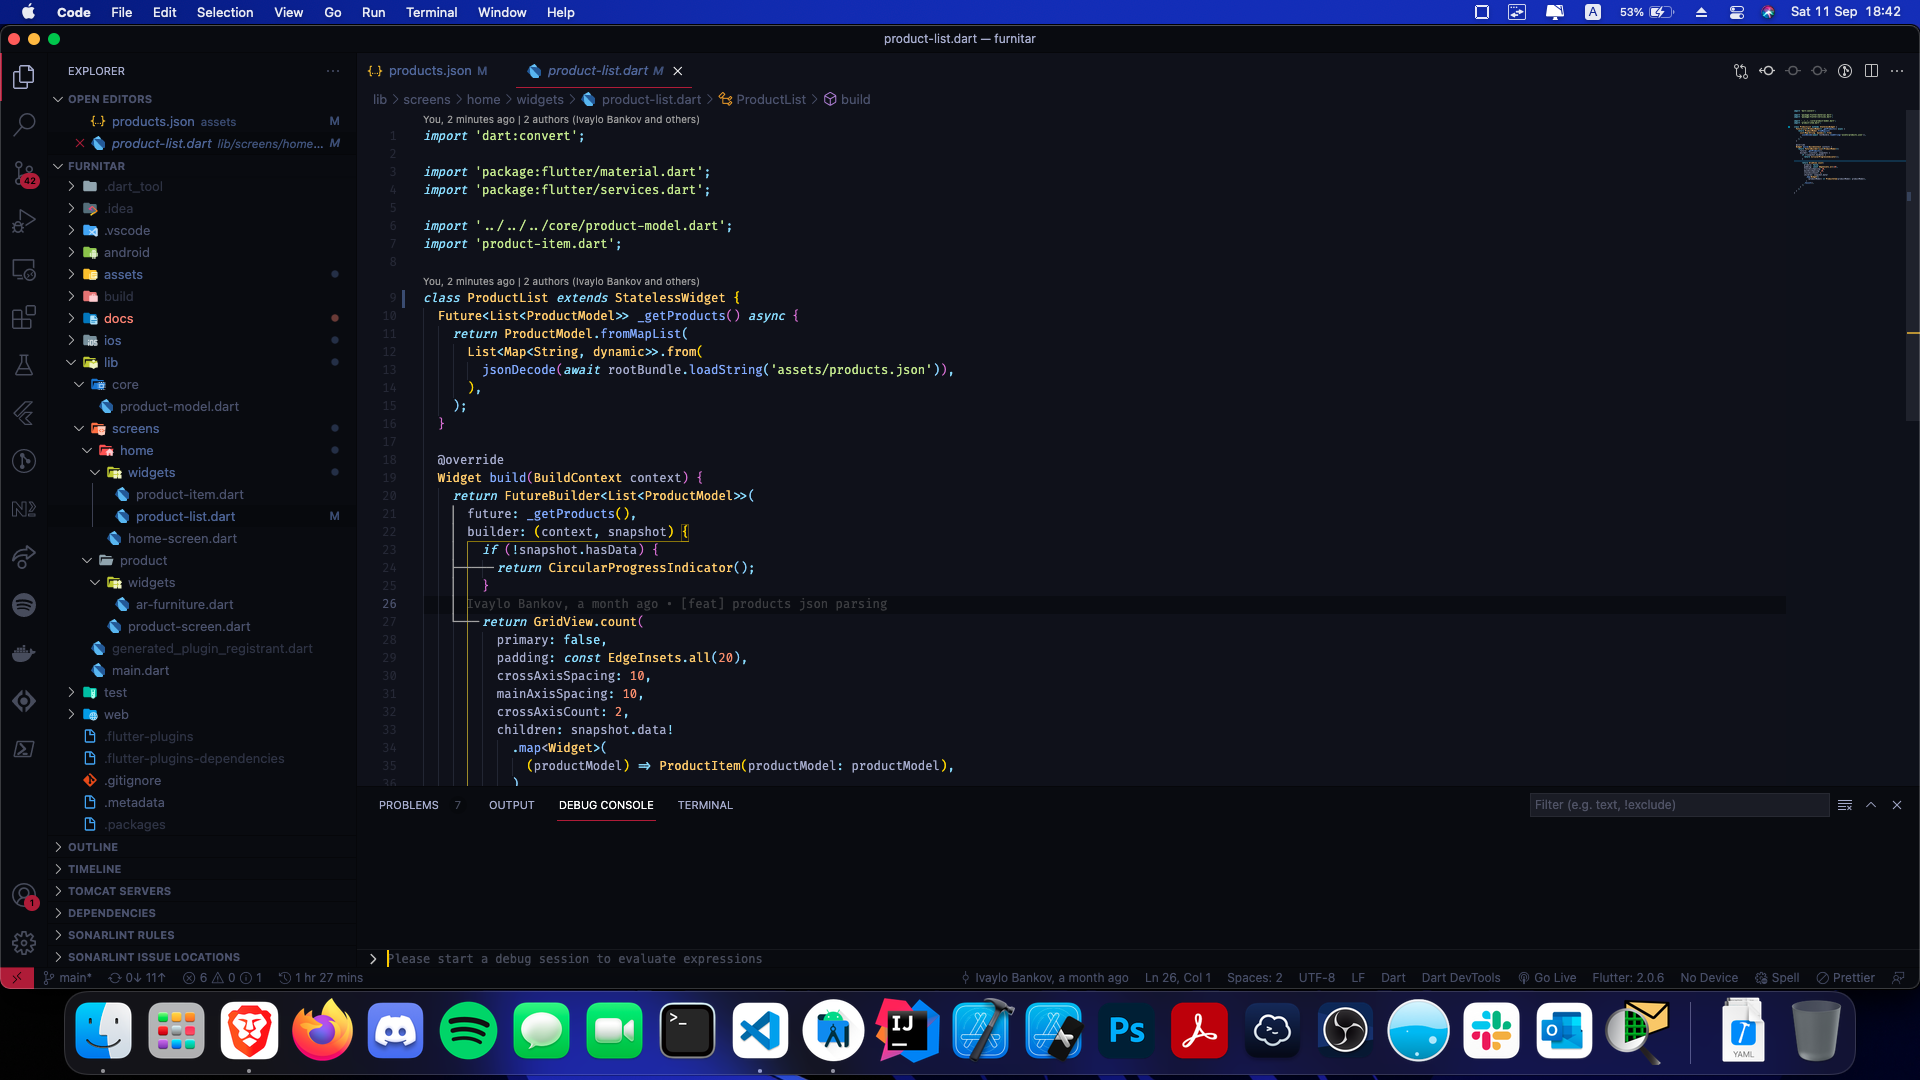
\includegraphics[width=1\textwidth]{screenshot-vscode.png}
    \centering
    \caption{Снимка от Visual Studio Code}
    \label{fig:screenshot-vscode}
\end{figure}

\subsection{ARCore}
ARCore, известен също като Google Play Services за AR, е комплект за разработка на софтуер, разработен от Google, който позволява да се създават приложения за разширена реалност. ARCore използва три ключови технологии за интегриране на виртуално съдържание с реалния свят, видян през камерата на Android мобилното устройство:

\begin{itemize}
    \item Т.нар ``Шест степени на свобода'' (на англ. ``Six degrees of freedom'') позволяват на телефона да разбира и проследява позицията си спрямо света.
    \item Екологичното разбиране, наблюдавано от телефона, позволява на телефона да открива размера и местоположението на плоски хоризонтални повърхности като земята или масичка за кафе.
    \item Оценката на светлината позволява на телефона да прецени текущите условия на осветеност на околната среда.
\end{itemize}

ARCore е интегриран в множество мобилни Android устройства. (Фиг. \ref{fig:arcore-arkit-logos})

\subsection{ARKit}
ARKit съчетава проследяване на движението на iOS устройствата, заснемане на камера, усъвършенствана обработка на сцени и удобства на дисплея, за да опрости задачата за изграждане на AR приложения. Технологията може да създава много видове AR с тези технологии, като се използва предната или задната камера на iOS устройство. (Фиг. \ref{fig:arcore-arkit-logos})

\begin{figure}[H]
    
\includegraphics[width=0.45\textwidth]{arcore-logo.png}
    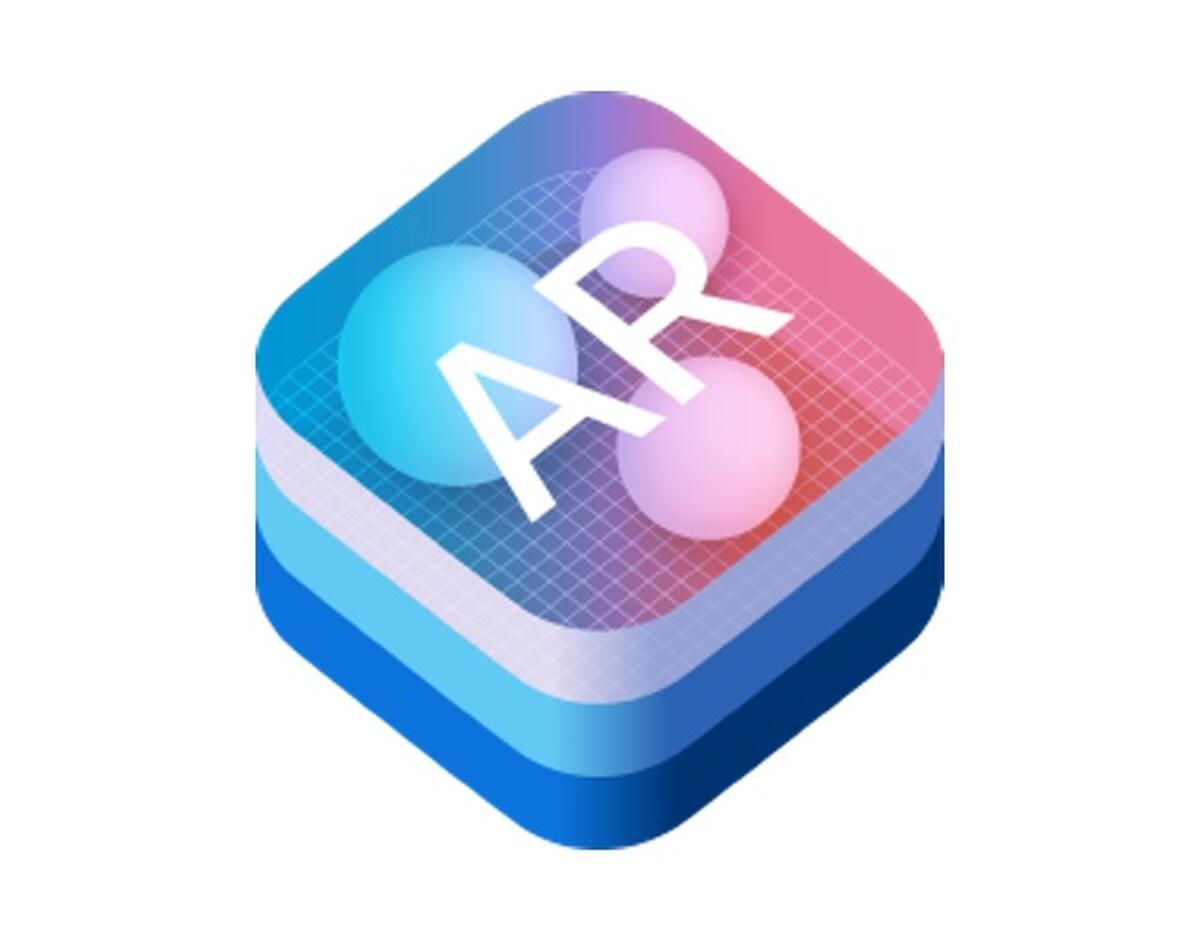
\includegraphics[width=0.45\textwidth]{arkit-logo.jpeg}
    \centering
    \caption{Логота на ARCore и ARKit}
    \label{fig:arcore-arkit-logos}
\end{figure}

\subsection{XML}
Extensible Markup Language (накратко XML) е стандарт (метаезик), дефиниращ правила за създаване на специализирани маркиращи езици, както и синтаксисът, на който тези езици трябва да се подчиняват. В последните няколко години, XML губи популярност като формат за съхранение на данни и бива заменен от JSON. (Фиг. \ref{fig:example-xml})

\begin{figure}[H]
    \lstinputlisting[language=XML]{code/example.xml}
    \centering
    \caption{Примерен XML документ}
    \label{fig:example-xml}
\end{figure}

\subsection{JSON}
JavaScript Object Notation (накратко JSON), е текстово базиран отворен стандарт създаден за човешки четим обмен на данни. Произлиза от скриптовия език JavaScript, за да представя прости структури от данни и асоциативни масиви, наречени обекти. Въпреки своята връзка с JavaScript, това е езиково независима спецификация, с анализатори, които могат да преобразуват много други езици в JSON. Основно JSON се използва при разработката на REST приложнопрограни интерфейси. (Фиг. \ref{fig:example-json})

\begin{figure}[H]
    \lstinputlisting[language=Java]{code/example.json}
    \centering
    \caption{Примерен JSON документ}
    \label{fig:example-json}
\end{figure}
